\documentclass[border=10pt]{standalone}
\usepackage{tikz}
\usetikzlibrary{shapes,arrows,positioning,calc}

\begin{document}
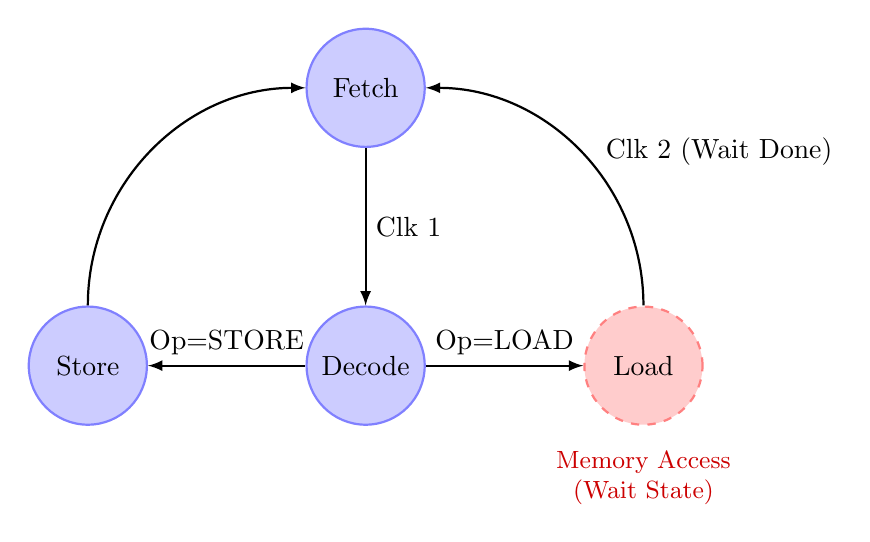
\begin{tikzpicture}[
    node distance=2.5cm,
    state/.style={circle, draw=blue!50, fill=blue!20, thick, minimum size=1.5cm, text centered},
    wait/.style={circle, draw=red!50, fill=red!20, thick, minimum size=1.5cm, text centered, dashed},
    arrow/.style={->, >=latex, thick, auto}
]

% Nodes
\node [state] (fetch) {Fetch};
\node [state, below=2cm of fetch] (decode) {Decode};
\node [wait, right=2cm of decode] (load) {Load};
\node [state, left=2cm of decode] (store) {Store};

% Transitions
\draw [arrow] (fetch) -- (decode) node[midway, right] {Clk 1};
\draw [arrow] (decode) -- (load) node[midway, above] {Op=LOAD};
\draw [arrow] (decode) -- (store) node[midway, above] {Op=STORE};

% Return paths with bends to avoid crossing
\draw [arrow] (load) to [out=90, in=0] node[midway, right, xshift=0.2cm] {Clk 2 (Wait Done)} (fetch);
\draw [arrow] (store) to [out=90, in=180] (fetch);

% Annotation
\node [below=0.2cm of load, text width=3cm, align=center, font=\small, color=red!80!black] {Memory Access\\(Wait State)};

\end{tikzpicture}
\end{document}
